
\section{Physics Triggers}
\label{sec:physics_triggers}


\subsection{Electron Trigger}
\label{sec:electron_trigger}

The electron trigger is designed to select the inclusive electron scattering from the CLAS12 targets:
\begin{equation}
e(p,n,A)\rightarrow e^\prime X.
\label{eqn:electron}
\end{equation}
\noindent
The trigger  selects  events with at least one scattered electron detected by the forward detectors. The High Threshold Cherenkov Counter (HTCC),  Preshower Calorimeter (PCAL),  Electromagnetic Calorimeter (EC), and Drift Chambers (DC) participate in the generation of the trigger decision. Searching for the electrons is performed  in all six CLAS12 sectors in parallel. The final electron trigger is  a simple "OR" of the six sector trigger signals.

The HTCC discriminates electrons from other charged particles. This detector must be calibrated in terms of the number of photoelectrons before the start of any experiment. The HTCC trigger logic  searches for clusters and calculates the total number of  photoelectrons  detected by the HTCC. The cluster may include up to four PMT signals that collect the Cherenkov light from the adjacent mirrors as described in Section ~\ref{sec:HTCC}. The minimum number of  photoelectrons in the cluster  is one of the main electron trigger parameters. Usually this threshold is set to 1-2 photoelectrons depending on the experiment requirements.

The PCAL and EC calorimeters are designed to detect photons and electrons as described in Section ~\ref{sec:ECAL}. A high energy deposition in the calorimeters is a signature of electron detection, and is one of the electron trigger parameters. The PCAL and EC detectors must be calibrated before the start of any experiment in terms of energy deposition measured in MeV. The electron trigger uses cuts on the cluster energy in the PCAL ($E_{PCAL}$) and EC ($E_{EC}$) separately, and cuts on the total energy deposition in both detectors $E_{Total}=E_{PCAL}+E_{EC}$.
These cuts   depend  on the beam energy and the experiment requirements, and usually lie in the region  150-300~MeV (corresponding to minimum electron energy from 600-1200~MeV) for the energy sum $E_{Total}$.

Geometrical matching between the HTCC signal and the position of the shower in the PCAL calorimeter helps to suppress
random coincidences between the two detectors. The trigger firmware uses the HTCC-PCAL look-up table to make a proper event selection.

The track reconstruction in the DC system at the trigger level is very useful for the further suppression of accidental background, as described in Section ~\ref{sec:DC}. The trigger decision requires at least 3 layers in every superlayer and at least 5 superlayers in every road, which is a standard setting for all triggers where the DC-based component is used. The geometrical matching between track candidates and hits in the PCAL and EC detectors is used to strengthen the trigger performance in terms of event purity.



\begin{figure}[!htb]
 	\centering
  	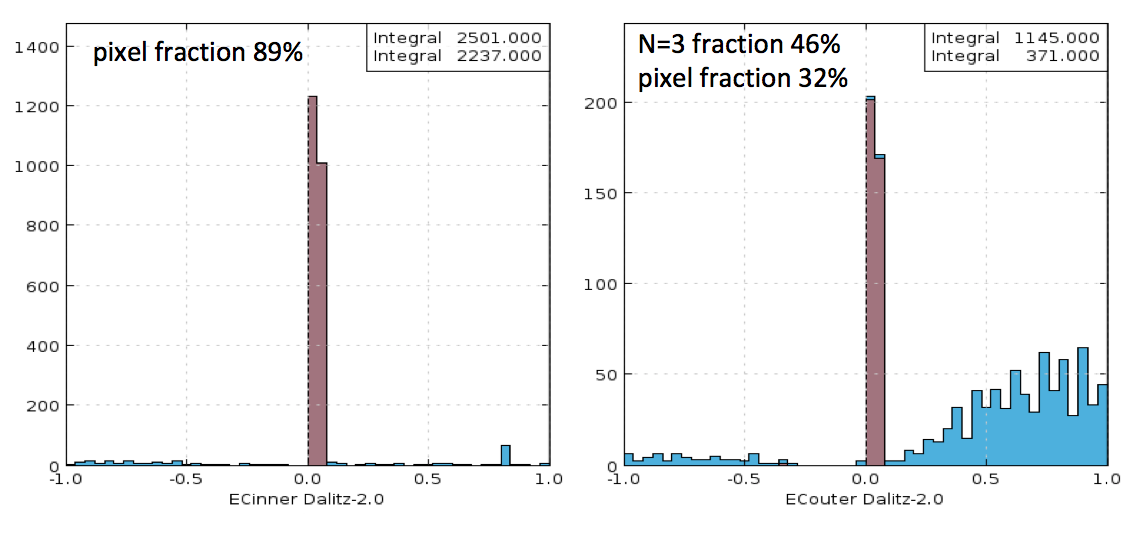
\includegraphics[width=1.0\columnwidth,keepaspectratio]{img/PixelFraction.png}
 	\caption{Offline analysis of events that satisfied the pixel trigger on $EC_{inner}$  calorimeter.  Left plot shows 89$\%$ of $EC_{inner}$  triggers satisfied the pixel test $dU+dV+dW=2$.  Right plot shows only 14$\%$ of the $EC_{inner}$ triggers found an $EC_{outer}$ event that satisfied both the $N=3$ and pixel test.}
	\label{fig:rlectron}
\end{figure}


\begin{figure}[!htb]
 	\centering
  	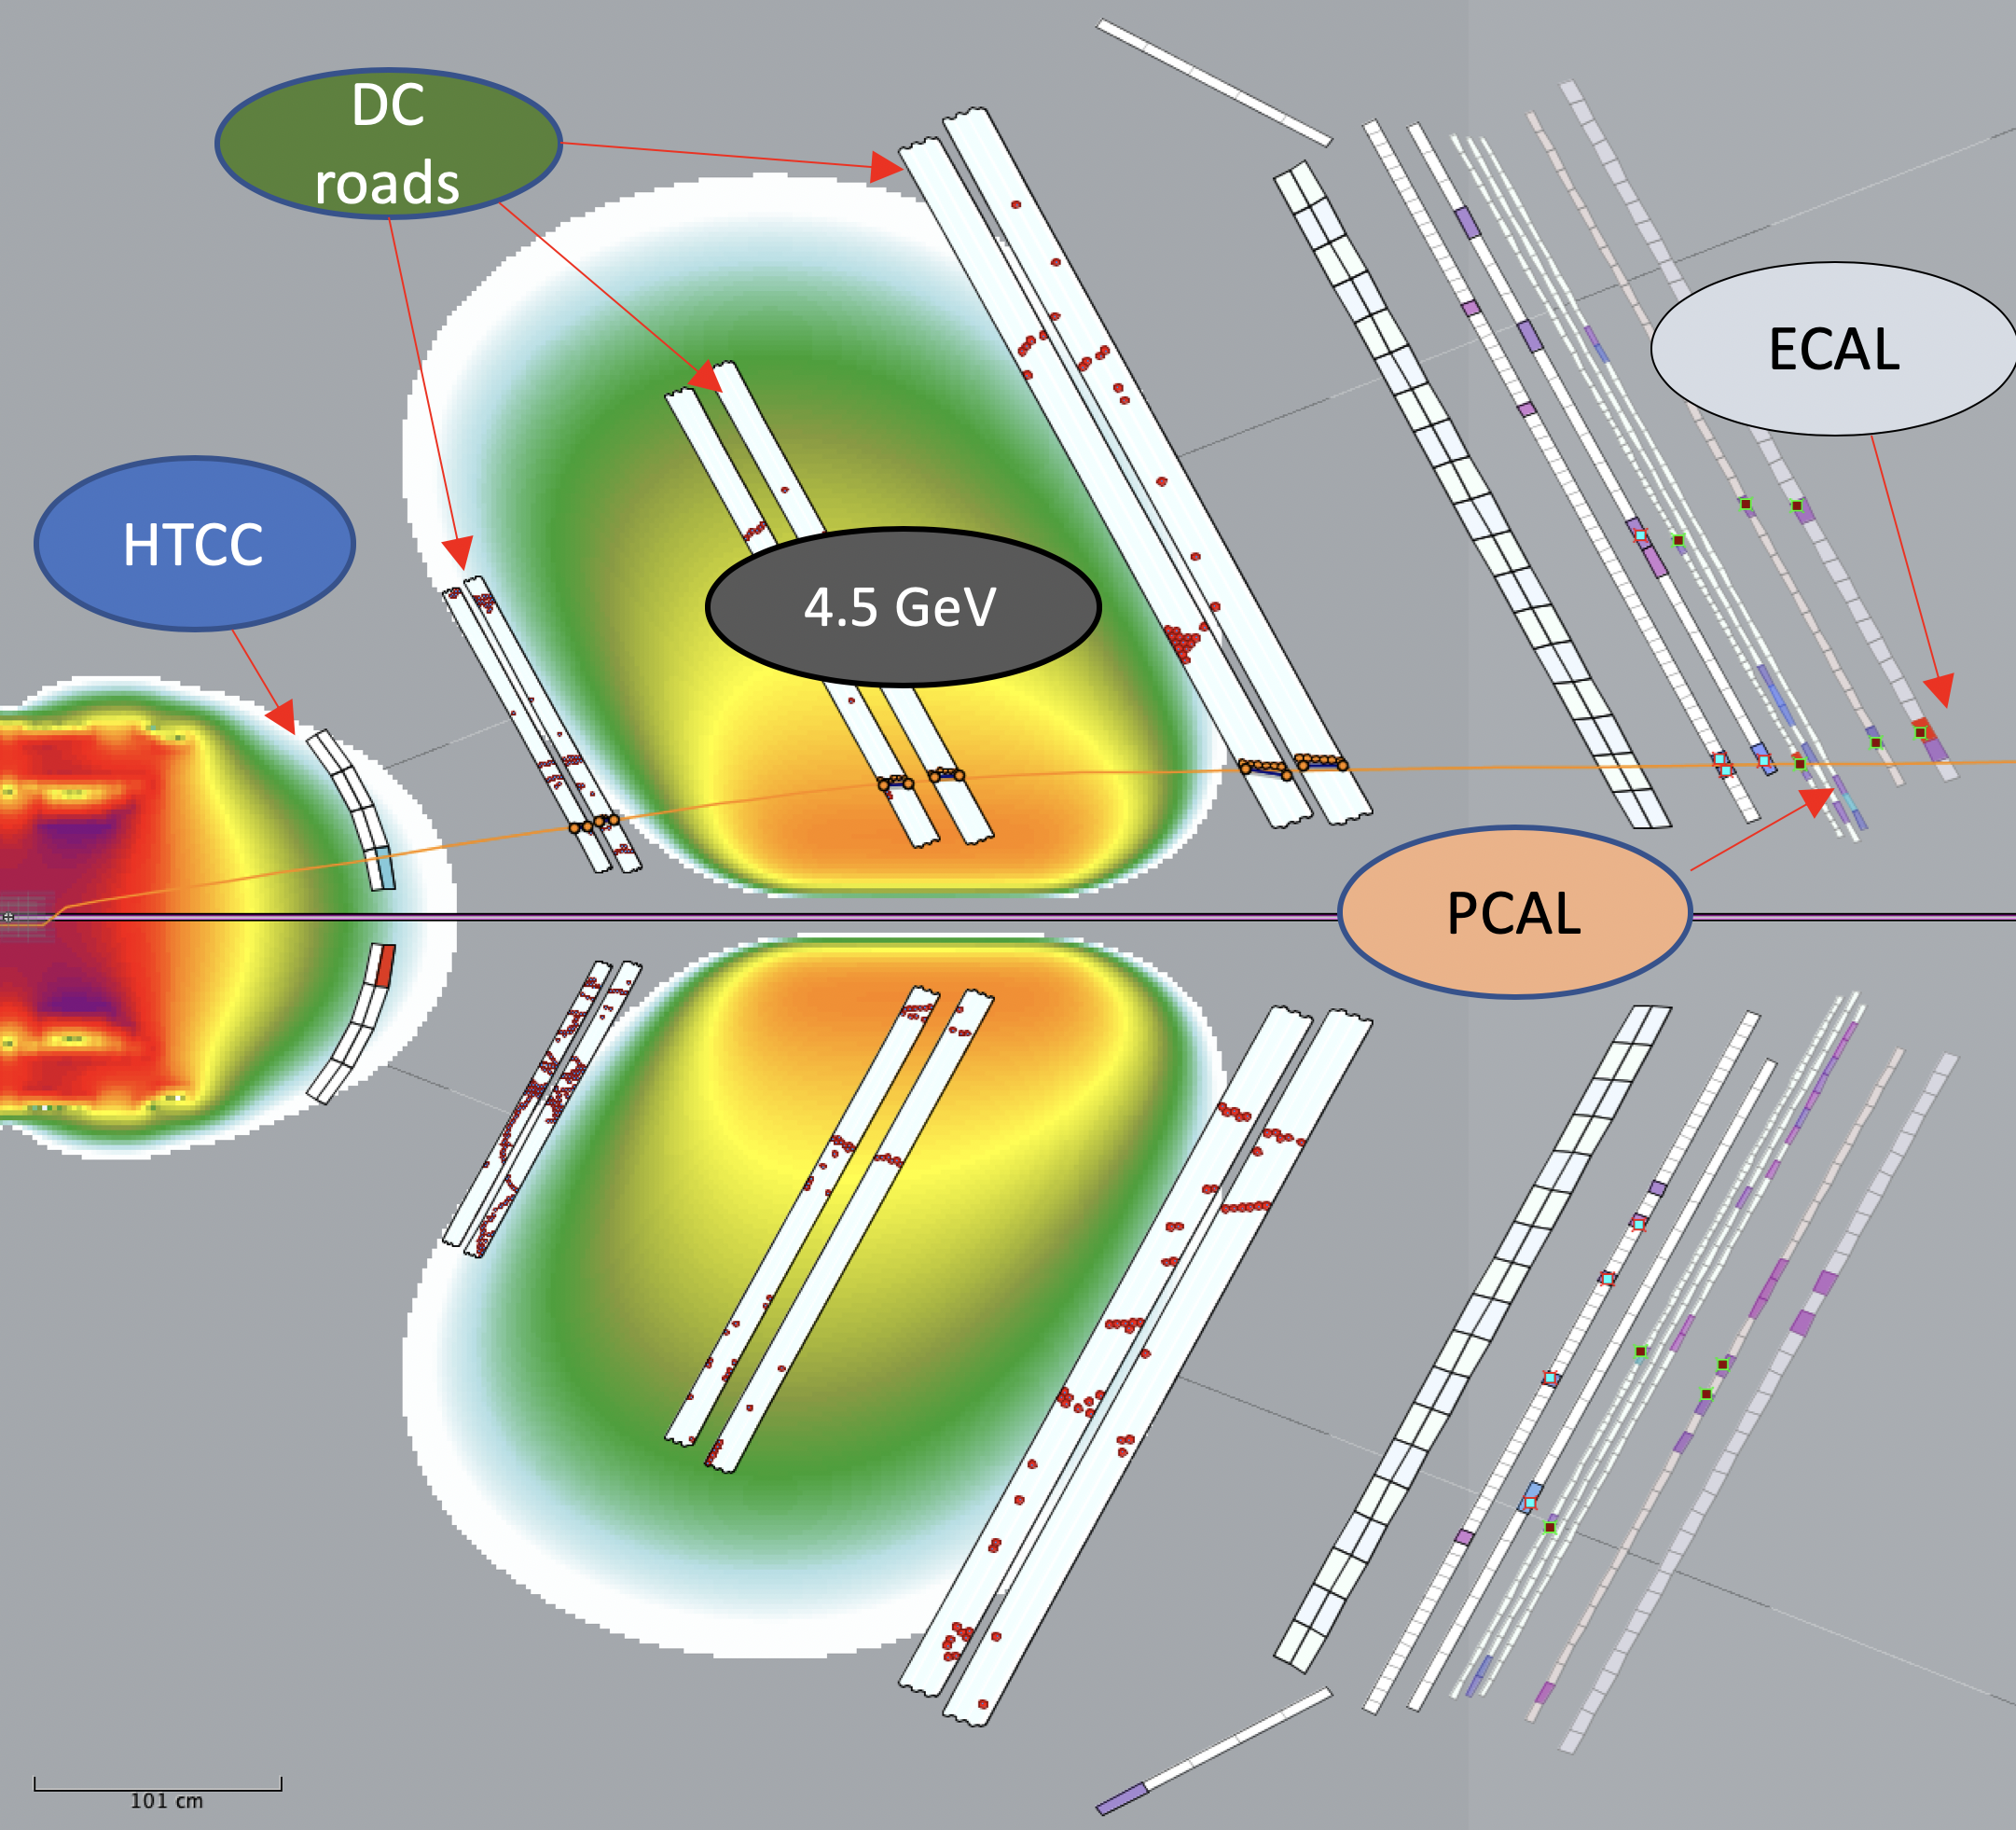
\includegraphics[width=0.95\columnwidth,keepaspectratio]{img/Electron_trigger.png}
 	\caption{(Color online) Display of the event selected by the electron trigger. The trigger detectors HTCC, DC, PCAL and ECAL are indicated in the picture. The electron momentum is 4.5 GeV/c.}
	\label{fig:electron}
\end{figure}

The electron trigger configuration may be represented by the formula:
\begin{align} 
\label{eq:em_trg_formula}
\begin{split}
 & HTCC_i(N_{phe}{>}N^{HTCC}_{min})\times\\
 & [E_{PCAL}{>}E^{PCAL}_{min}) \times E_{Total}{>}E^{Total}_{min})\times  DC]_i
 \end{split}
\end{align}
\noindent
where index $i$ is the CLAS12 sector number and $N_{phe}$ is the number of photoelectrons detected by the HTCC in a defined cluster. $N^{HTCC}_{min}$,  $E^{PCAL}_{min}$, $ E^{Total}_{min}$ are trigger parameters, and $DC$ means that  a track was reconstructed by the $DC$-system. The space correlations between all detectors and coordinates of the track are implemented as well. The event display with the 4.5 GeV/c electron, selected by the trigger, is shown in Fig.~\ref{fig:electron}.


\subsection{Photoproduction Trigger}
\label{sec:photoproduction_trigger}

The photoproduction trigger is designed to select events where a scattered electron is detected by the Forward Tagger in the polar angular range from 2$\degree$ to 5$\degree$. Strictly speaking it is not a photoproduction process but electron scattering with low four-momentum transfer $Q^2=4E_{beam}E'\sin^2\theta/2$. The trigger logic continuously searches for clusters in the FT calorimeter from an electromagnetic shower, and calculates the shower energy and space coordinates. The cluster energy is the sum of all  crystal energies within a 3x3 spatial array that meet the time-matching constraints. Once the clustering algorithm  has identified a cluster, the corresponding data is reported to the next trigger stage. This includes the timestamp, the energy, and the spatial coordinates (center of the seed crystal). The cluster energy is not corrected for shower leakage effects at this stage. Finally, the trigger processor makes the trigger decision by applying further cuts to the clusters. The trigger  selection is based on lower and upper energy limits and the number of hits in the cluster. The trigger may also select events with a specified number of clusters detected by the calorimeter.  The coincidence with the two-plane  scintillating hodoscope $FTHodo$,  located in front of the calorimeter, serves to discriminate charged particles from high-energy photons. The geometry matching between FT cluster and $FTHodo$ hit helps to suppress background coming from photons.  The trigger logics also provides  the possibility to select reactions with an electron and several photons in the final state, for example
$$
ep\to e'\gamma\gamma X.
$$
\noindent
The display of two events with  one and two clusters in the Forward calorimeter, selected by the Forward tagger trigger, is shown in Fig.~\ref{fig:FT_trigger}.

The Trigger System may use the  information from the CLAS12 Forward and Central Detectors to select events with several charged or neutral particles in coincidence with the electron in the FT calorimeter. The trigger detector composition depends on the reaction under study. 

Charged particles in the Forward Detectors are selected by a coincidence between the FTOF, PCAL, and EC with tracks reconstructed by the DC system. The space correlations between all trigger detectors are required, including coordinates of tracks crossing the detector planes. Hit matching along the track is an important part of the background reduction at the trigger level. The cuts on the energy depositions in the trigger detectors are used to select charged and neutral particles. 

 \begin{figure}[!htb]
 	\centering
  	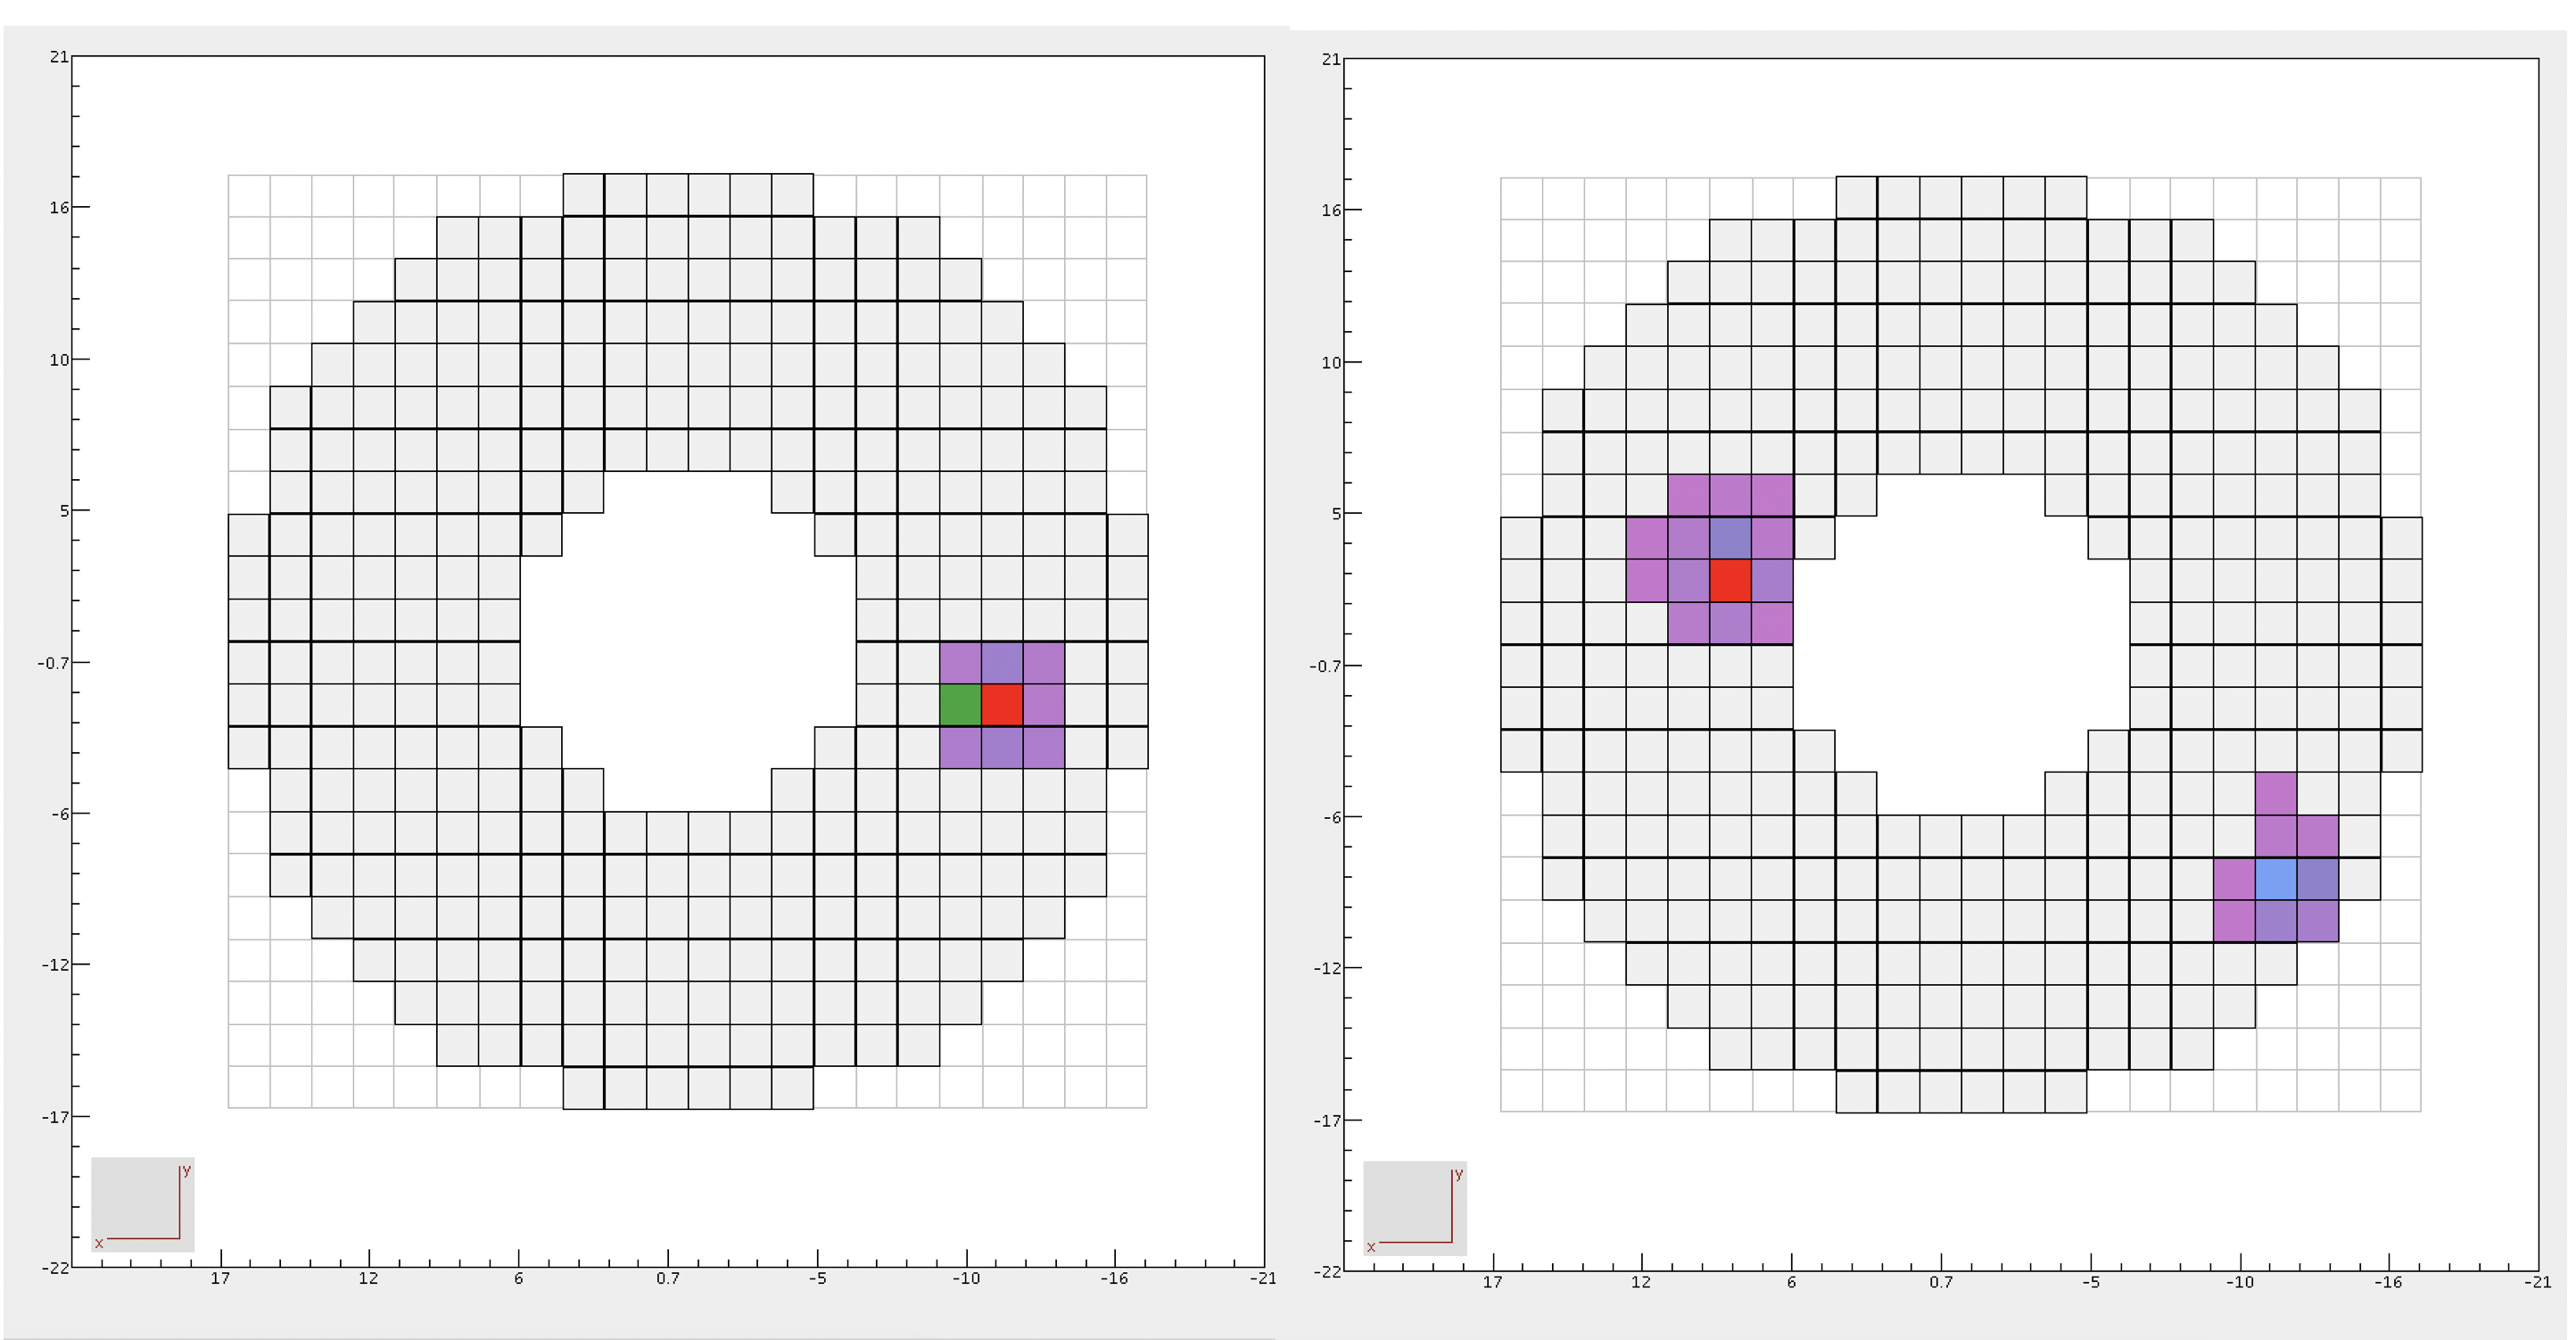
\includegraphics[width=0.95\columnwidth,keepaspectratio]{img/FT_trigger.png}
 	\caption{(Color online) Display of two events, selected by the Forward Tagger trigger, with one and two clusters in the Forward calorimeter.}
	\label{fig:FT_trigger}
\end{figure}

 The trigger configuration 
 \begin{align*} 
 &FT(E^{FT}_{min}{<}E{<}E^{FT}_{max})\times FTHodo(2)\times\\
 & [FTOF(E{>}E^{FTOF}_{min})\times PCAL(E{>}E^{PCAL}_{min})\times  DC]_i
\end{align*}
was used in the first CLAS12 experiments to select the reaction 
$$ep\to e'h^{+/-}_F X$$
 with at least one electron and one particle $h^{+/-}_F$ with a definite charge in the final state.  The charge of the particle is the trigger parameter. Trigger can select negative, positive or just   particle with any  charge in the final state.
$FTHodo(2)$ denotes the inclusion of the hodoscope to the trigger with hits in both planes, correlated  in space with FT cluster. 
The index $i$ denotes the CLAS12 sector number. Each detector has its own trigger energy cuts: $ E^{FT}_{min}$,  $E^{FT}_{max}$, $E^{FTOF}_{min}$, and $E^{PCAL}_{min}$. A space correlation matching requirement between the FTOF and PCAL elements was implemented. The trigger rate was too high for the available DAQ bandwidth, so this trigger was prescaled. 

The selection of the events with at least one electron and two charged particles in the forward direction detected in different sectors
$$
ep\to e' h^{+/-}_F h^{+/-}_F X.
$$ 
was done by the trigger configuration
 \begin{align*} 
 &FT(E^{FT}_{min}{<}E{<}E^{FT}_{max}) \times FTHodo(2)\times\\
 & [FTOF(E{>}E^{FTOF}_{min})\times  PCAL(E{>}E^{PCAL}_{min})\times   DC]_i \times \\
 & [FTOF(E{>}E^{FTOF}_{min})\times  PCAL(E{>}E^{PCAL}_{min})\times   DC]_j,
\end{align*}
where $i$ and $j$ denote different CLAS12 sectors. 
 
The central detectors, such as Central Time-of-Flight (CTOF) and Central Neutral Detector (CND), were used for the selection of the events with at least one  particle detected in the Central Detector. 
The trigger configuration
 \begin{align*} 
 &FT(E^{FT}_{min}{<}E{<}E^{FT}_{max}) \times FTHodo(2)\times\\
 & [FTOF(E{>}E^{FTOF}_{min})\times  PCAL(E{>}E^{PCAL}_{min})\times   DC]_i \times \\
 & CTOF(E{>}E^{CTOF}_{min})\end{align*}
\noindent
was used for the selection of events with an electron in the FT, at least one charged paticle going in the forward direction, and at least one particle detected in the central detectors. 
$$
ep\to e' h^{+/-}_F  h^{+/-}_C X.
$$
$h^{+/-}_C$ stands for the charge particle in the Central Detector.
\noindent
The CND detector could be  added to the coincidence chain with the space correlation between the CTOF and CND counters in case the triger rate is too high
 \begin{align*} 
 &FT(E^{FT}_{min}{<}E{<}E^{FT}_{max})\times FTHodo(2)\times \\
 & [FTOF(E{>}E^{FTOF}_{min})\times  PCAL(E{>}E^{PCAL}_{min})\times   DC]_i \times \\
 & CTOF(E{>}E^{CTOF}_{min})\times  CND(E{>}E^{CND}_{min}).
\end{align*}
\noindent
As stated above, the minimum energy depositions in all detectors in the trigger are parameters that depend on the individual experiment requirements.


\subsection{$J/\psi$ Meson Trigger}
\label{sec:meson_trigger}
A special trigger was designed to detect the quasi-photoproduction of $J/\psi$-mesons
$$
ep \to e' J/\psi p', J/\psi \to \mu^+\mu^-
$$
Two decay modes are useful for the selection of the $J/\psi$ meson: $J/\psi \to e^+e^-$ and $J/\psi \to \mu^+\mu^-$.
The conventional electron and photoproduction triggers  select the $J/\psi$-meson  in case of the decay to the electron-positron pair. However, these trigger configurations do not  work  with muons in the final state. Therefore, another trigger was added to select one more decay mode for this experiment. The CLAS12 spectrometer has no dedicated muon system, but it turns out that the selection of particles with energy deposition in the PCAL-EC calorimeters close to the minimum-ionizing  value is sufficient to suppress the background from pions when the invariant mass of the two particles (muons or pions) is near the $J/\psi$-mass. The muons from the $J/\psi$ decay appear in opposite CLAS12 sectors, which allowed for the trigger configuration:  
\begin{align*} 
 & [FTOF(E{{>}}5){\times}  PCAL(15{<}E{<}60){\times} \\
 & {\qquad} EC(60{<}E{<}120){\times}   DC]_i {\times} \\
 & [FTOF(E{{>}}5){\times}  PCAL(15{<}E{<}60){\times} \\
 & {\qquad} EC(60{<}E{<}120){\times}   DC]_j  
\end{align*}
\noindent
The energy units are in MeV. Note, that there is no requirement to search for the scattered electron at all. This gives an order of magnitude advantage in the  virtual photon flux in comparison with the case when the electron is detected in the FT calorimeter.
\begin{figure}[!htb]
 	\centering
  	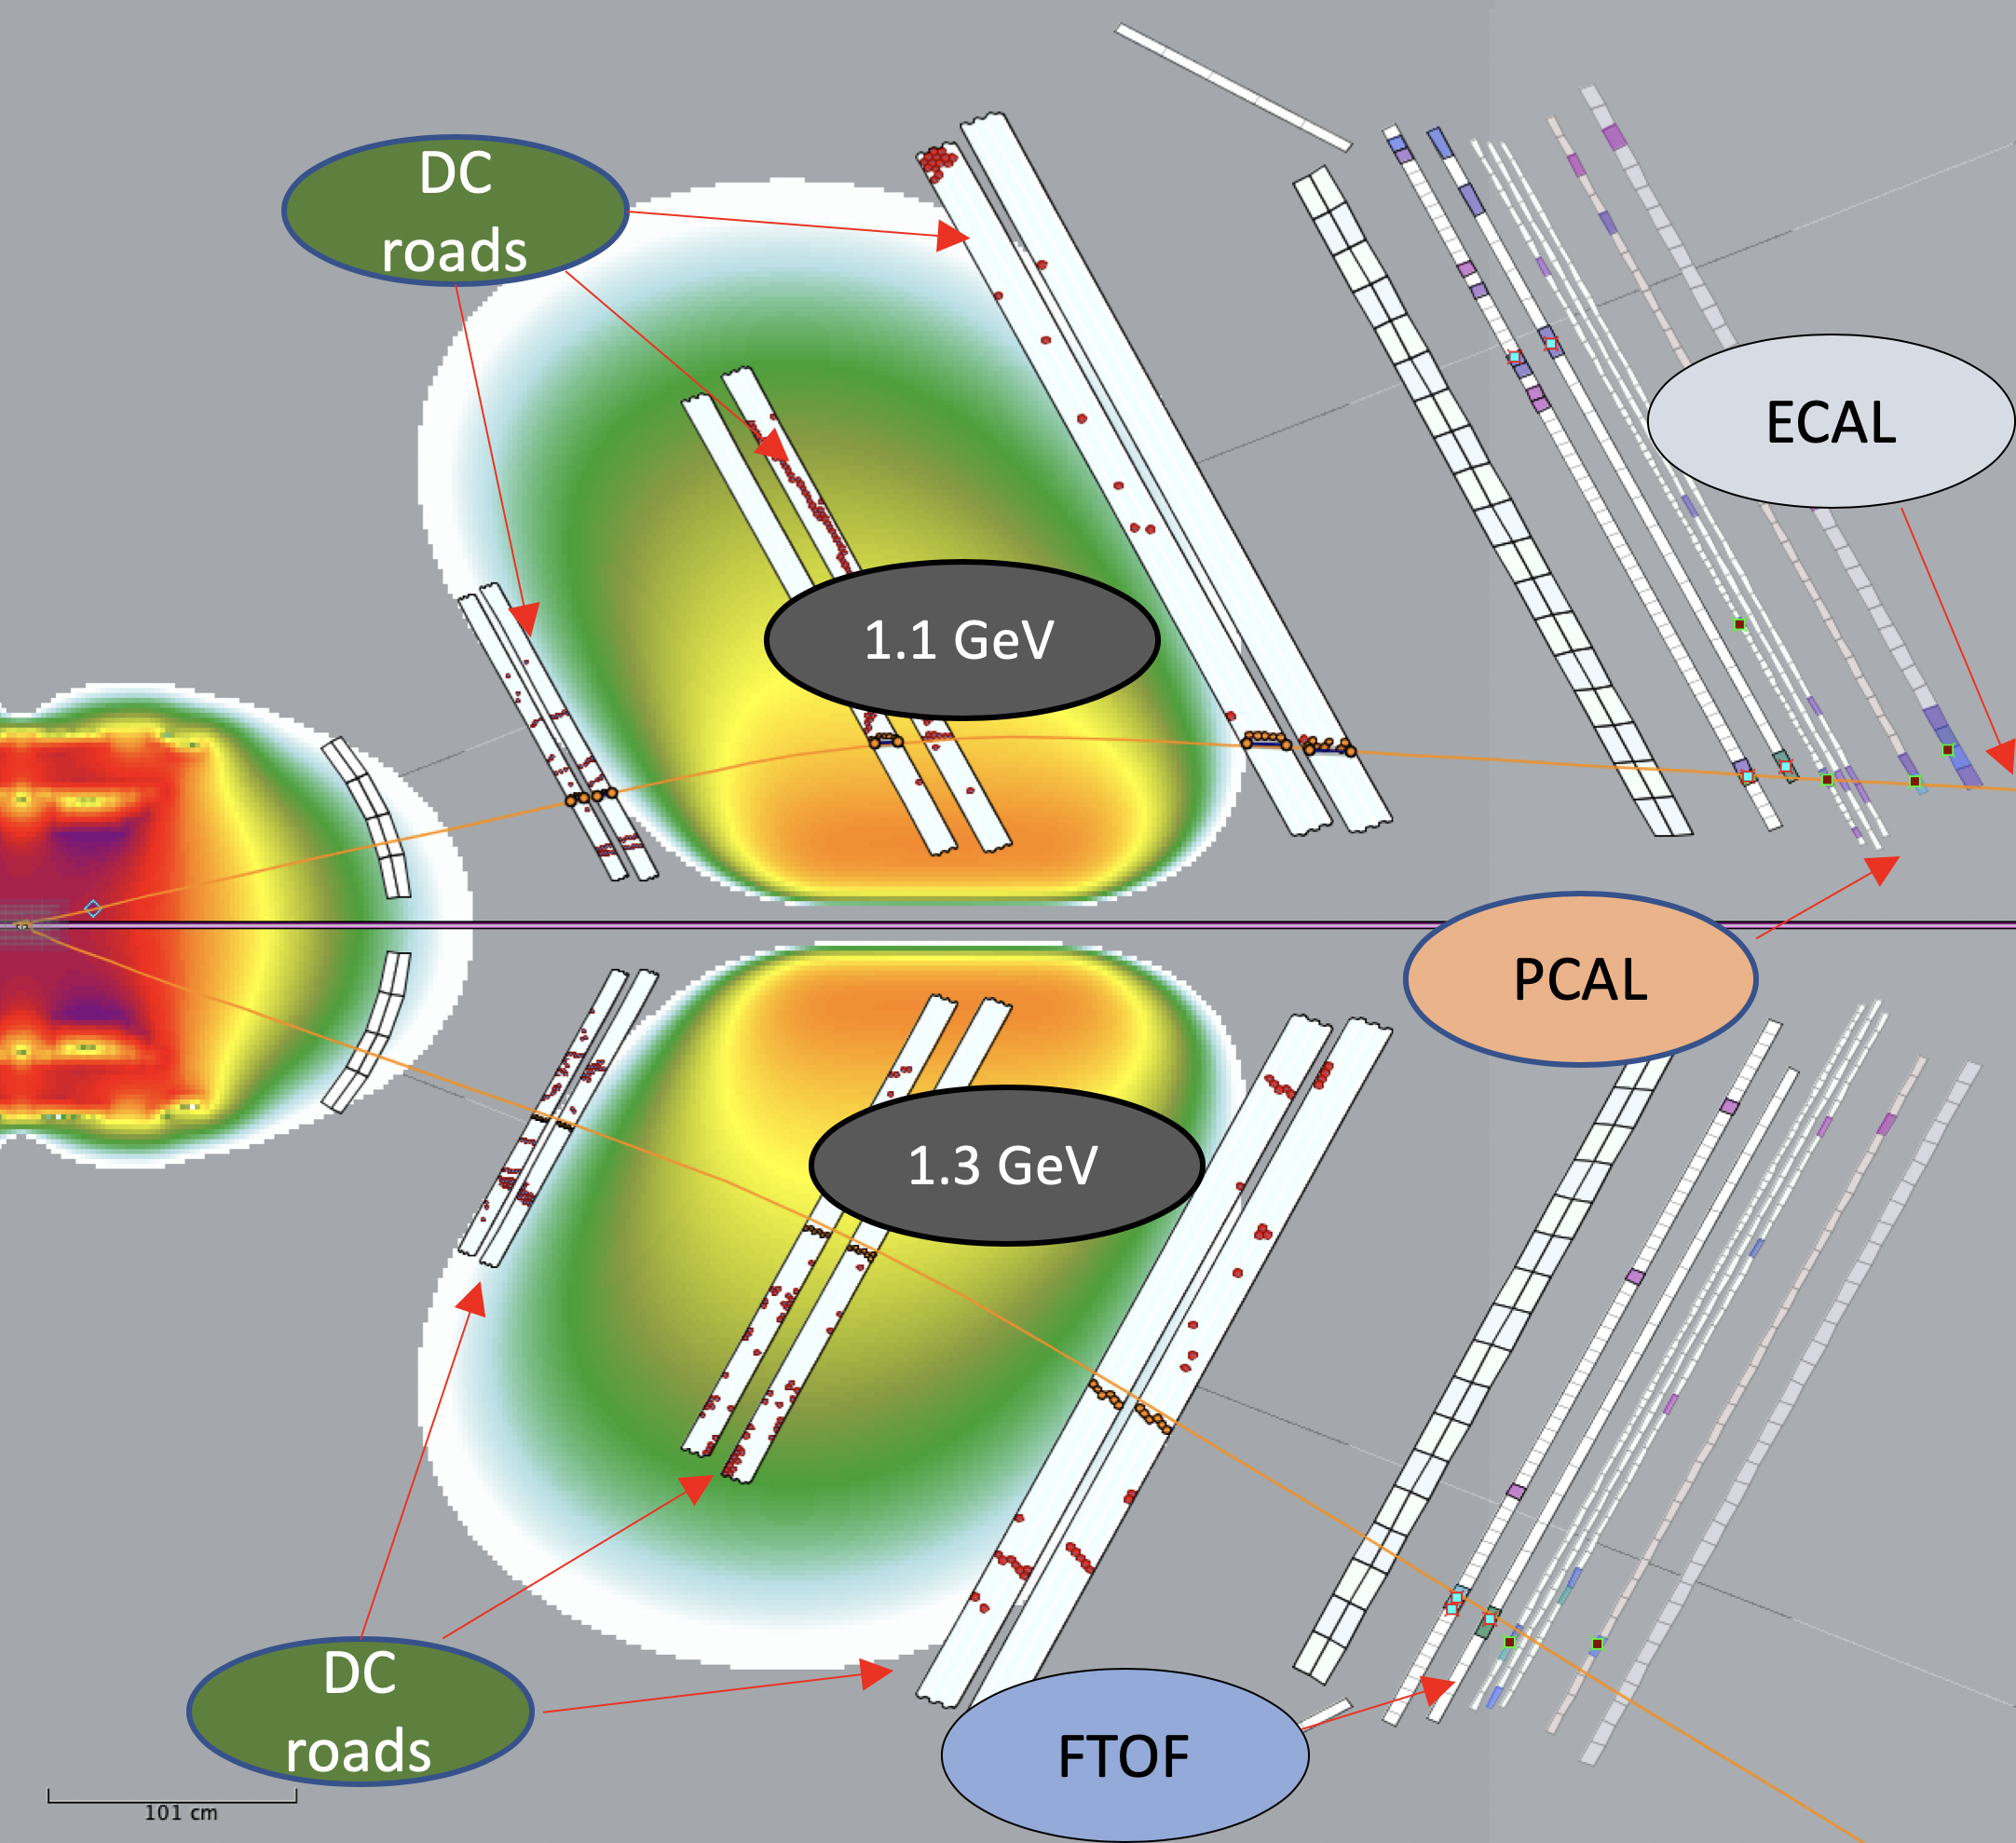
\includegraphics[width=0.95\columnwidth,keepaspectratio]{img/Muon_trigger.png}
 	\caption{(Color online) Display of event selected by the muon trigger. The trigger detectors DC, FTOP, PCAL and ECAL are indicated in the picture. The particle momenta are  1.1 and 1.3 GeV/c.}
	\label{fig:muon}
\end{figure}
\noindent
 The event display with  two particles with opposite charges and in the opposite sectors, selected by muon trigger, is shown in Fig.~\ref{fig:muon}.



